\documentclass[aspectratio=169]{beamer}

% ---------- ENCODING & FONTS ----------
\usepackage[utf8]{inputenc}
\usepackage[T1]{fontenc}

% ---------- THEME & LOOK ----------
\usetheme{Madrid}
\usecolortheme{seahorse}
\usefonttheme{professionalfonts}
\setbeamertemplate{navigation symbols}{}
\setbeamercovered{transparent}
\setbeamertemplate{itemize items}[circle]
\setbeamertemplate{enumerate items}[default]
\setlength{\parskip}{0.25em}

% ---------- COLORS ----------
% Beamer already loads xcolor, so we just define our colors
\definecolor{accent}{RGB}{0,92,184}
\definecolor{soft}{RGB}{233,244,255}
\definecolor{lightred}{RGB}{245,210,210}
\setbeamercolor{structure}{fg=accent}
\setbeamercolor{title}{fg=white,bg=accent}
\setbeamercolor{frametitle}{fg=accent}
\setbeamercolor{block title}{bg=accent!12,fg=accent}
\setbeamercolor{block body}{bg=soft}

% ---------- PACKAGES ----------
\usepackage{booktabs}
\usepackage{amsmath, amssymb}
\usepackage{array}
\usepackage{multirow}
\usepackage{hyperref}
\hypersetup{colorlinks=true,linkcolor=accent,urlcolor=accent}

% ---------- SAFE TRANSITION FALLBACK ----------
\makeatletter
\@ifundefined{transfade}{\newcommand{\transfade}[1][]{}}{}
\makeatother

% ---------- PLACEHOLDER BOX FOR FIGURES ----------
\newcommand{\placeholderbox}[2][0.82\linewidth]{%
  \begin{center}
    \fbox{\begin{minipage}[c][0.46\textheight][c]{#1}
      \centering \vspace{0.3em}
      \textbf{#2}\\[0.6em]
      \emph{Insert figure/diagram here later.}
    \end{minipage}}
  \end{center}
}

% ---------- TITLE ----------
\title{\textbf{Aggregate Expenditure and Output in the Short Run \vspace{.5cm}\\  }}
\subtitle{ {\large ECON 101 - Macroeconomics}}
%\institute{UNBC}
\author{Muhebullah Karimzada}
\date{Winter 2026}

\begin{document}

% ============================================================
% TITLE
% ============================================================
\begin{frame}[plain]
  \titlepage
\end{frame}

% ============================================================
\begin{frame}{Chapter Outline}
\transfade
\begin{itemize}[<+->]
  \item \textbf{8.1} The Aggregate Expenditure Model
  \item \textbf{8.2} Determining Aggregate Expenditure in the Economy
  \item \textbf{8.3} Graphing Macroeconomic Equilibrium
  \item \textbf{8.4} The Multiplier Effect
  \item \textbf{8.5} The Aggregate Demand Curve
  \item \textbf{Appendix} The Algebra of Macroeconomic Equilibrium
\end{itemize}
\end{frame}

% ============================================================
\section{8.1 The Aggregate Expenditure Model}
% ============================================================

\begin{frame}{8.1 Learning Objective}
\transfade
\begin{block}{Goal}
Understand how macroeconomic equilibrium is determined in the aggregate expenditure model.
\end{block}
\begin{itemize}[<+->]
  \item We build a simple short-run model called the \textbf{aggregate expenditure (AE) model}.
  \item It focuses on the relationship between:
  \begin{itemize}[<+->]
    \item total spending (\textbf{aggregate expenditure}) and
    \item output (\textbf{real GDP}),
  \end{itemize}
  \item assuming the \textbf{price level is constant} in the short run.
\end{itemize}
\end{frame}

\begin{frame}{Aggregate Expenditure: Definition}
\transfade
\begin{itemize}[<+->]
  \item \textbf{Aggregate expenditure (AE):} total planned spending in the economy.
  \item Components:
  \begin{align*}
    AE &= C + I + G + NX
  \end{align*}
  \begin{itemize}[<+->]
    \item \(C\): consumption
    \item \(I\): planned investment
    \item \(G\): government purchases
    \item \(NX\): net exports (exports minus imports)
  \end{itemize}
  \item In this model we study how changes in these components affect equilibrium real GDP.
\end{itemize}
\end{frame}

\begin{frame}{Four Components of Aggregate Expenditure}
\transfade
\begin{itemize}[<+->]
  \item \textbf{Consumption (C):}
  \begin{itemize}[<+->]
    \item Spending by households on goods and services.
  \end{itemize}
  \item \textbf{Planned investment (I):}
  \begin{itemize}[<+->]
    \item Planned spending by firms on capital goods (machinery, buildings, equipment),
    \item plus planned spending by households on new homes.
  \end{itemize}
  \item \textbf{Government purchases (G):}
  \begin{itemize}[<+->]
    \item Government spending on goods and services at all levels (federal, provincial, local),
    \item excluding transfer payments.
  \end{itemize}
  \item \textbf{Net exports (NX):}
  \begin{itemize}[<+->]
    \item Value of exports minus the value of imports.
  \end{itemize}
\end{itemize}
\end{frame}

\begin{frame}{Planned Investment vs. Actual Investment}
\transfade
\begin{itemize}[<+->]
  \item National accounts measure \textbf{actual investment}.
  \item In the AE model we focus on \textbf{planned investment}:
  \begin{itemize}[<+->]
    \item Investment firms intend to carry out.
  \end{itemize}
  \item \textbf{Actual investment} includes:
  \begin{itemize}[<+->]
    \item planned investment plus
    \item \textbf{unplanned inventory changes} (changes in unsold goods).
  \end{itemize}
  \item In the AE model:
  \begin{itemize}[<+->]
    \item Planned investment does not include unplanned changes in inventories.
  \end{itemize}
\end{itemize}
\end{frame}

\begin{frame}{Macroeconomic Equilibrium in the AE Model}
\transfade
\begin{itemize}[<+->]
  \item \textbf{Macroeconomic equilibrium} occurs when:
  \[
    \text{Planned aggregate expenditure} = \text{Real GDP}.
  \]
  \item If planned spending is greater than output:
  \begin{itemize}[<+->]
    \item firms sell more than expected,
    \item inventories fall,
    \item firms respond by increasing production and employment.
  \end{itemize}
  \item If planned spending is less than output:
  \begin{itemize}[<+->]
    \item firms sell less than expected,
    \item inventories rise,
    \item firms respond by reducing production and employment.
  \end{itemize}
\end{itemize}
\end{frame}

\begin{frame}{Table 8.1 -- Planned AE, GDP, and Inventories}
\centering
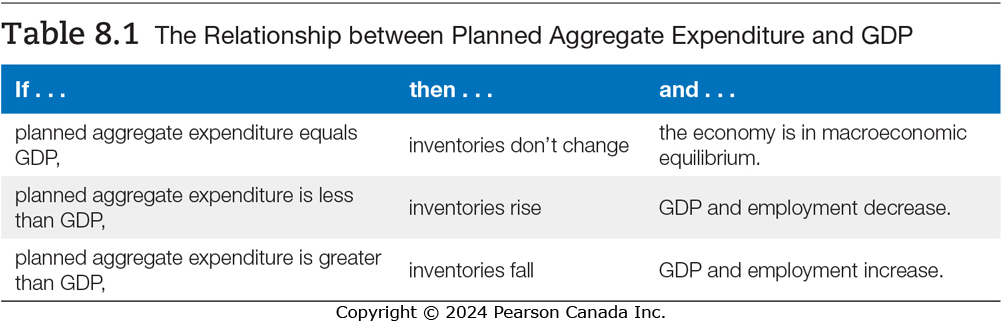
\includegraphics[width=0.91\linewidth]{Tab08-001}.
\end{frame}

\begin{frame}{Table 8.2 -- Components of AE, 2021}
\centering
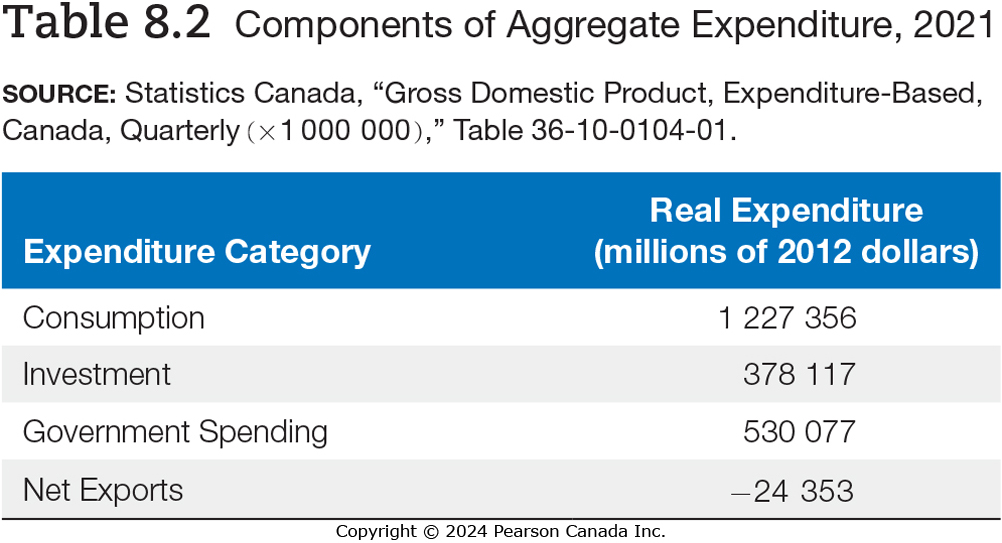
\includegraphics[width=0.91\linewidth]{Tab08-002}.
\end{frame}

% ------------------------------------------------------------
% Consumption and Its Determinants
% ------------------------------------------------------------

\begin{frame}{Figure 8.1 -- Real Consumption }
\centering
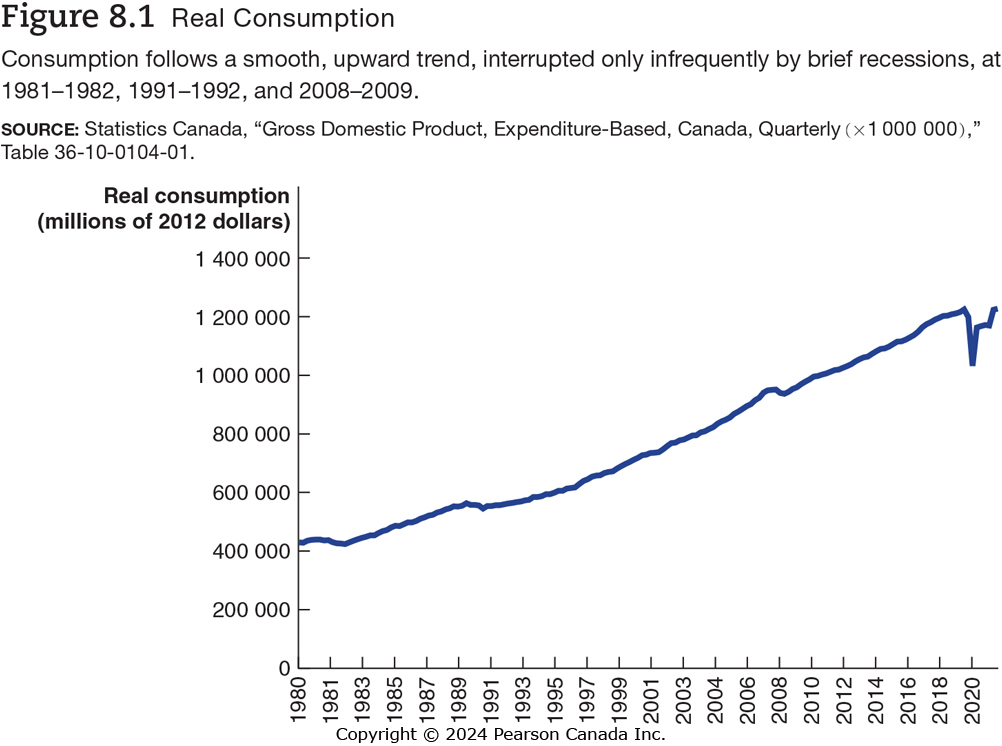
\includegraphics[width=0.81\linewidth]{Fig08-001}.
\end{frame}

\begin{frame}{Determinants of Consumption (1 of 2)}
\transfade
\begin{itemize}[<+->]
  \item \textbf{Current disposable income}
  \begin{itemize}[<+->]
    \item Main driver of consumer spending.
    \item Higher after-tax income \(\Rightarrow\) higher consumption.
  \end{itemize}
  \item \textbf{Household wealth}
  \begin{itemize}[<+->]
    \item Wealth = assets (homes, stocks, bonds, bank accounts) minus liabilities (mortgages, loans).
    \item Wealthier households tend to spend more at any given income level.
    \item Empirical estimates: a permanent \$1 increase in wealth raises annual consumption by a few cents.
  \end{itemize}
\end{itemize}
\end{frame}

\begin{frame}{Determinants of Consumption (2 of 2)}
\transfade
\begin{itemize}[<+->]
  \item \textbf{Expected future income}
  \begin{itemize}[<+->]
    \item Households prefer \textbf{consumption smoothing}.
    \item They base current spending partly on what they expect to earn in the future.
  \end{itemize}
  \item \textbf{Price level}
  \begin{itemize}[<+->]
    \item Higher price level reduces the real value of wealth.
    \item With the same dollar wealth, households can buy fewer goods and services \(\Rightarrow\) lower consumption.
  \end{itemize}
  \item \textbf{Interest rate}
  \begin{itemize}[<+->]
    \item Higher real interest rate encourages saving and discourages borrowing.
    \item Especially reduces spending on durable goods (cars, appliances, houses).
  \end{itemize}
\end{itemize}
\end{frame}

\begin{frame}{Consumption and Consumer Confidence}
\transfade
\begin{itemize}[<+->]
  \item Consumer spending also depends on how people feel about the future.
  \item \textbf{Consumer confidence} indices summarize:
  \begin{itemize}[<+->]
    \item expectations about income, employment, and overall economic conditions.
  \end{itemize}
  \item When confidence rises:
  \begin{itemize}[<+->]
    \item households are more willing to spend,
    \item AE shifts upward.
  \end{itemize}
  \item When confidence falls:
  \begin{itemize}[<+->]
    \item households cut back on spending,
    \item AE shifts downward.
  \end{itemize}
\end{itemize}
\end{frame}

\begin{frame}{Figure 8.2 -- Consumption and Income, 1981–2020 }
\centering
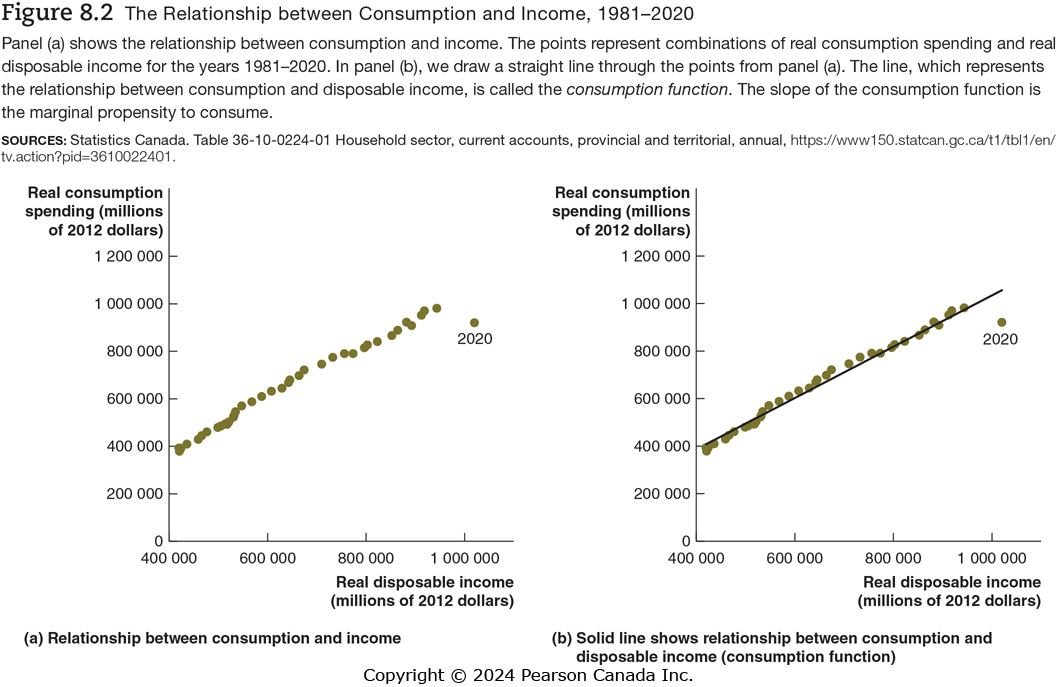
\includegraphics[width=0.84\linewidth]{Fig08-002}.
\end{frame}

% ------------------------------------------------------------
% Consumption Function, MPC, and MPS
% ------------------------------------------------------------

\begin{frame}{The Consumption Function and MPC}
\transfade
\begin{itemize}[<+->]
  \item The \textbf{consumption function} describes how consumption depends on disposable income:
  \[
    C = C_0 + \text{MPC} \times Y_{\text{D}},
  \]
  where:
  \begin{itemize}[<+->]
    \item \(C_0\) = autonomous consumption,
    \item \(Y_{\text{D}}\) = disposable income,
    \item \(\text{MPC}\) = marginal propensity to consume.
  \end{itemize}
  \item \textbf{Marginal propensity to consume (MPC):}
  \[
    \text{MPC} =
    \frac{\Delta C}{\Delta Y_{\text{D}}}.
  \]
  \item It measures how much consumption changes when disposable income changes by one dollar.
\end{itemize}
\end{frame}

\begin{frame}{MPC: Numerical Example}
\transfade
\begin{itemize}[<+->]
  \item Suppose data suggest that when disposable income rises by \$10{,}000:
  \begin{itemize}[<+->]
    \item consumption rises by about \$7{,}640.
  \end{itemize}
  \item Then:
  \[
    \text{MPC} \approx \frac{7{,}640}{10{,}000} = 0.764.
  \]
  \item Interpretation:
  \begin{itemize}[<+->]
    \item Households spend about \alert{76.4\%} of each additional dollar of income on consumption,
    \item and save the remaining \(\approx 23.6\%\).
  \end{itemize}
\end{itemize}
\end{frame}

\begin{frame}{Consumption, National Income, and Saving}
\transfade
\begin{itemize}[<+->]
  \item For this chapter we treat:
  \[
    \text{National income} \approx Y \approx \text{real GDP}.
  \]
  \item Disposable income:
  \[
    Y_{\text{D}} = Y - T_{\text{net}},
  \]
  where \(T_{\text{net}}\) = taxes minus transfers.
  \item Any part of disposable income not spent is \textbf{saving}:
  \[
    Y_{\text{D}} = C + S.
  \]
\end{itemize}
\end{frame}

\begin{frame}{Figure 8.3 -- Consumption and National Income}
\centering
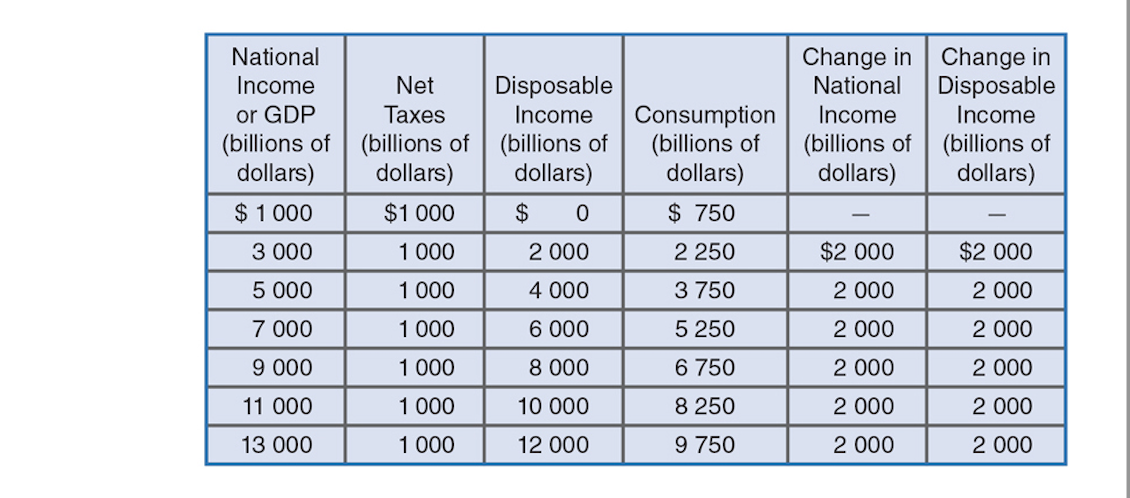
\includegraphics[width=0.95\linewidth]{Fig08-003a}.
\end{frame}

\begin{frame}{Figure 8.3 -- Consumption and National Income}
\centering
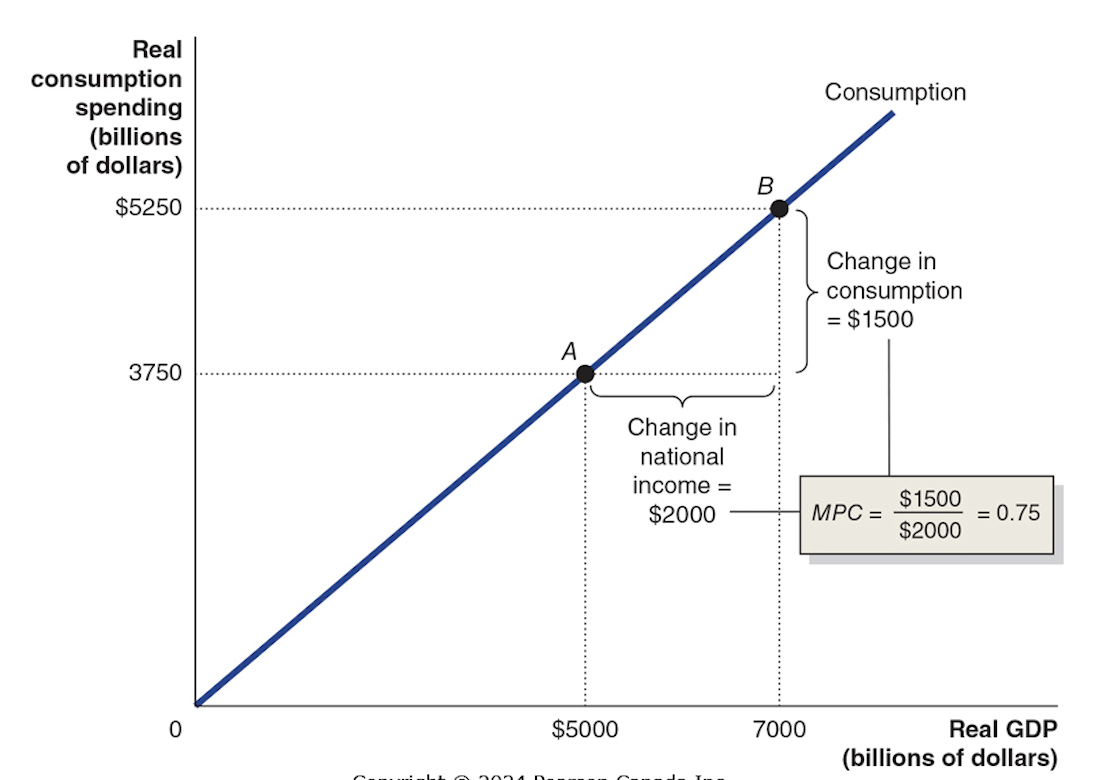
\includegraphics[width=0.7\linewidth]{Fig08-003b}.
\end{frame}

\begin{frame}{Income Changes: Decomposing the Effects}
\transfade
\begin{itemize}[<+->]
  \item We can express changes in income as:
  \[
    \Delta Y = \Delta C + \Delta S + \Delta T_{\text{net}}.
  \]
  \item We assume net taxes do not change with income in this simple model:
  \[
    \Delta T_{\text{net}} = 0.
  \]
  \item Then:
  \[
    \Delta Y = \Delta C + \Delta S.
  \]
  \item Dividing by \(\Delta Y\):
  \[
    1 = \frac{\Delta C}{\Delta Y} + \frac{\Delta S}{\Delta Y}.
  \]
\end{itemize}
\end{frame}

\begin{frame}{Marginal Propensity to Save}
\transfade
\begin{itemize}[<+->]
  \item \textbf{Marginal propensity to save (MPS):}
  \[
    \text{MPS} = \frac{\Delta S}{\Delta Y}.
  \]
  \item From the previous equation:
  \[
    1 = \text{MPC} + \text{MPS}.
  \]
  \item So:
  \[
    \text{MPS} = 1 - \text{MPC}.
  \]
  \item Interpretation:
  \begin{itemize}[<+->]
    \item Every extra dollar of income is either:
    \begin{itemize}[<+->]
      \item spent (MPC part) or
      \item saved (MPS part).
    \end{itemize}
  \end{itemize}
\end{itemize}
\end{frame}

% ------------------------------------------------------------
% Determinants of Planned Investment, G, NX
% ------------------------------------------------------------

\begin{frame}{Figure 8.4 -- Real Investment}
 \centering
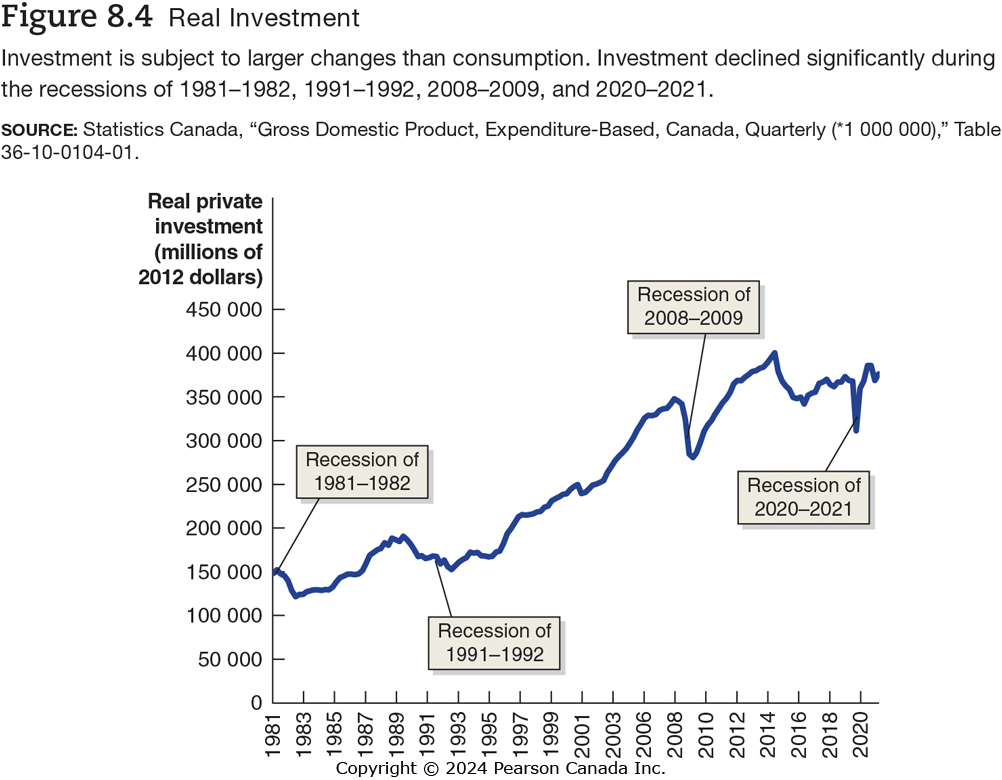
\includegraphics[width=0.64\linewidth]{Fig08-004}.

\end{frame}

\begin{frame}{Determinants of Planned Investment (1 of 2)}
\transfade
\begin{itemize}[<+->]
  \item \textbf{Expectations of future profits}
  \begin{itemize}[<+->]
    \item Capital goods and housing are long-lived.
    \item Firms invest more when they are optimistic about future profitability.
    \item Recessions and uncertainty reduce planned investment.
  \end{itemize}
  \item Purchases of new housing (by households) are part of planned investment:
  \begin{itemize}[<+->]
    \item When household wealth falls or income expectations weaken, new housing investment falls.
  \end{itemize}
\end{itemize}
\end{frame}

\begin{frame}{Determinants of Planned Investment (2 of 2)}
\transfade
\begin{itemize}[<+->]
  \item \textbf{Real interest rate}
  \begin{itemize}[<+->]
    \item Investment is often financed by borrowing.
    \item A higher real interest rate increases the cost of borrowing and reduces investment.
    \item A lower real interest rate encourages more investment.
  \end{itemize}
  \item \textbf{Taxes}
  \begin{itemize}[<+->]
    \item Higher corporate income taxes reduce after-tax profits and investment incentives.
    \item Investment tax credits can raise investment.
  \end{itemize}
  \item \textbf{Cash flow}
  \begin{itemize}[<+->]
    \item Many firms finance investment from internal funds (profits).
    \item Lower profits in recessions reduce cash flow and investment.
  \end{itemize}
\end{itemize}
\end{frame}

\begin{frame}{Figure 8.5 -- Real Government Purchases}
\centering
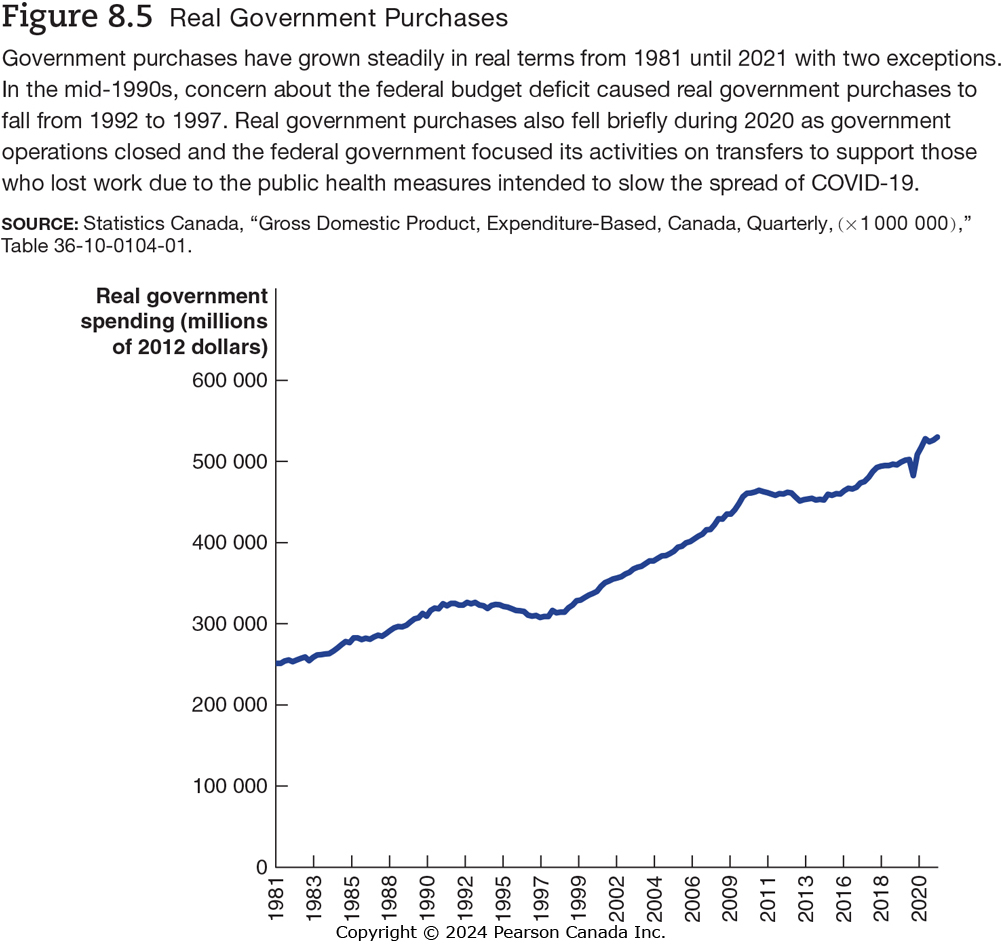
\includegraphics[width=0.6\linewidth]{Fig08-005}.
\end{frame}

\begin{frame}{Figure 8.6 -- Real Net Exports }
\centering
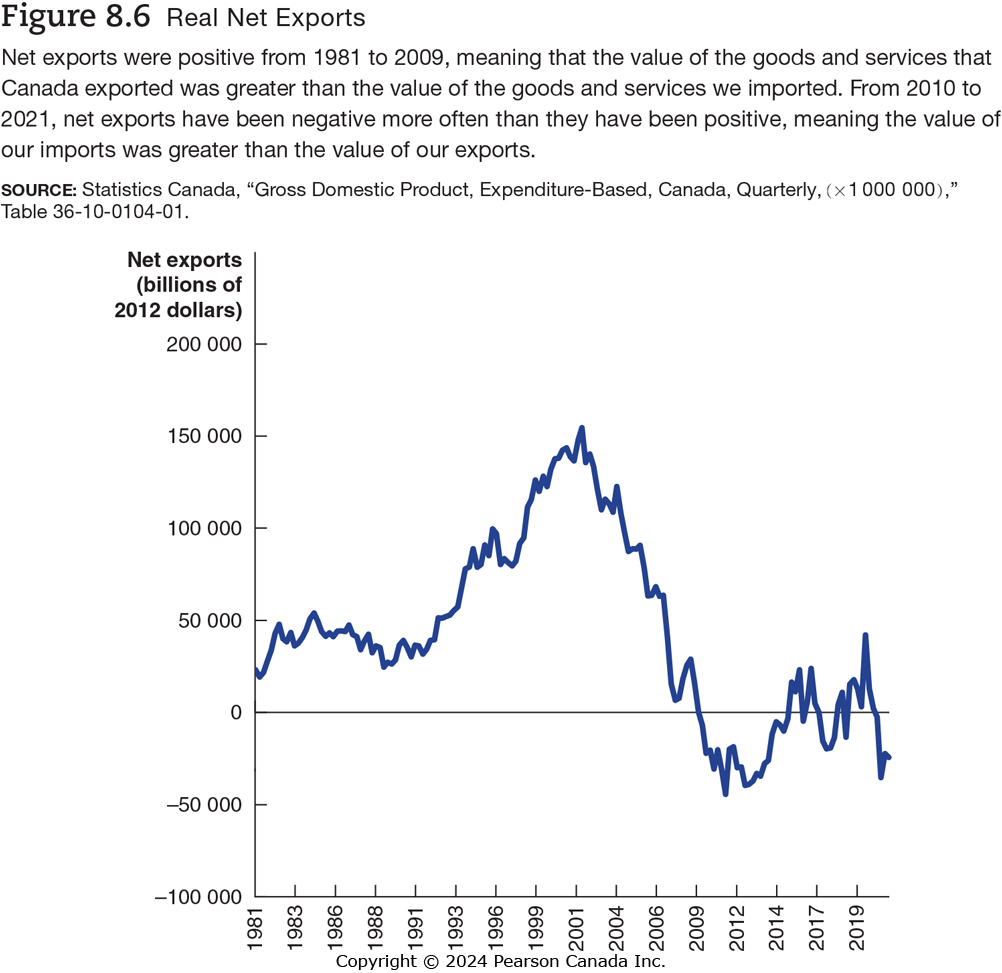
\includegraphics[width=0.56\linewidth]{Fig08-006}.
\end{frame}

\begin{frame}{Determinants of Net Exports}
\transfade
\begin{itemize}[<+->]
  \item Net exports depend on:
  \begin{itemize}[<+->]
    \item \textbf{Relative price levels}
      \begin{itemize}[<+->]
        \item If domestic prices rise faster than foreign prices, exports fall and imports rise.
      \end{itemize}
    \item \textbf{Relative growth rates}
      \begin{itemize}[<+->]
        \item If our economy grows faster than others, our imports tend to rise faster; exports may not keep up.
      \end{itemize}
    \item \textbf{Exchange rate}
      \begin{itemize}[<+->]
        \item A higher domestic currency value makes exports more expensive and imports cheaper \(\Rightarrow\) lower net exports.
      \end{itemize}
  \end{itemize}
\end{itemize}
\end{frame}

% ============================================================
\section{8.3 Graphing Macroeconomic Equilibrium}
% ============================================================

\begin{frame}{8.3 Learning Objective}
\transfade
\begin{block}{Goal}
Use a 45°-line diagram to illustrate macroeconomic equilibrium.
\end{block}
\begin{itemize}[<+->]
  \item We graph real GDP on the horizontal axis and \textbf{planned aggregate expenditure} on the vertical axis.
  \item The 45° line shows all points where:
  \[
    AE = Y.
  \]
\end{itemize}
\end{frame}

\begin{frame}{Figure 8.7 -- The 45°-Line Diagram }
\centering
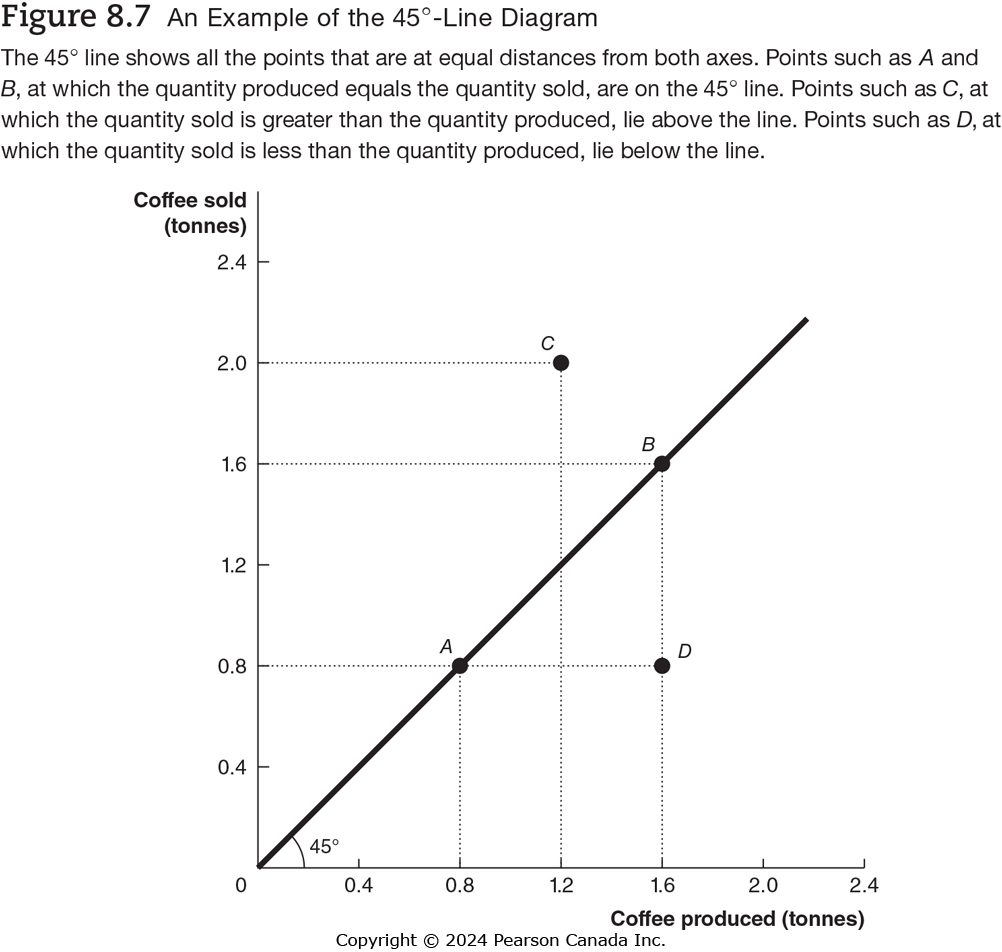
\includegraphics[width=0.5\linewidth]{Fig08-007}.
\end{frame}

\begin{frame}{Understanding the 45° Line}
\transfade
\begin{itemize}[<+->]
  \item On the 45° line:
  \[
    \text{Real GDP} = \text{Planned AE}.
  \]
  \item At a point like \textbf{C} (above 45° line):
  \begin{itemize}[<+->]
    \item Planned AE exceeds GDP,
    \item inventories fall,
    \item firms increase production \(\Rightarrow\) GDP rises toward equilibrium.
  \end{itemize}
  \item At a point like \textbf{D} (below 45° line):
  \begin{itemize}[<+->]
    \item Planned AE is less than GDP,
    \item inventories rise,
    \item firms cut production \(\Rightarrow\) GDP falls toward equilibrium.
  \end{itemize}
\end{itemize}
\end{frame}

\begin{frame}{Figure 8.8 -- AE and GDP in the 45° Diagram }
\centering
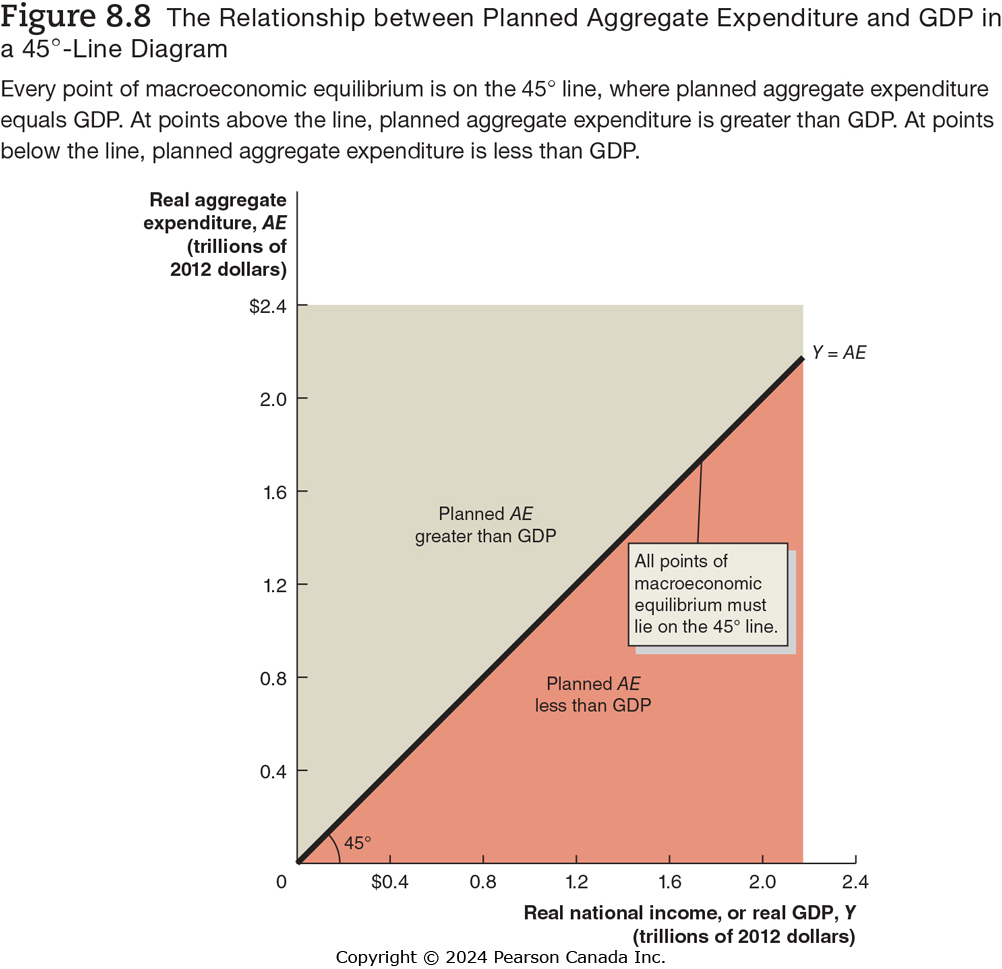
\includegraphics[width=0.48\linewidth]{Fig08-008}.
\end{frame}

\begin{frame}{Building the AE Line}
\transfade
\begin{itemize}[<+->]
  \item AE is built from its components:
  \[
    AE = C(Y) + I + G + NX.
  \]
  \item In this short-run model:
  \begin{itemize}[<+->]
    \item \(C\) increases with \(Y\),
    \item \(I, G, NX\) are taken as \textbf{autonomous} (do not change with income).
  \end{itemize}
  \item Graphically, AE is an upward-sloping line because:
  \begin{itemize}[<+->]
    \item higher income \(\Rightarrow\) higher consumption \(\Rightarrow\) higher AE.
  \end{itemize}
\end{itemize}
\end{frame}

\begin{frame}{Figure 8.9 -- Finding Macroeconomic Equilibrium}
\centering
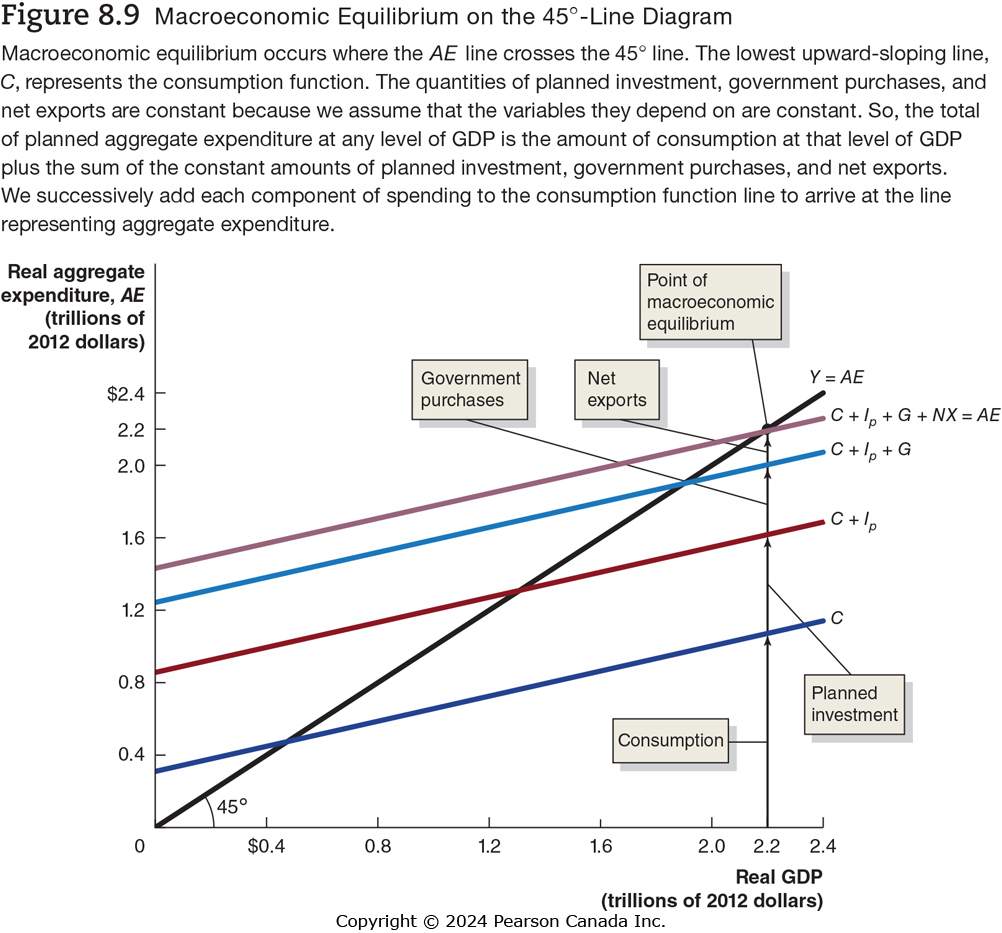
\includegraphics[width=0.6\linewidth]{Fig08-009}.
\end{frame}

\begin{frame}{Figure 8.10 -- Macroeconomic Equilibrium}
\centering
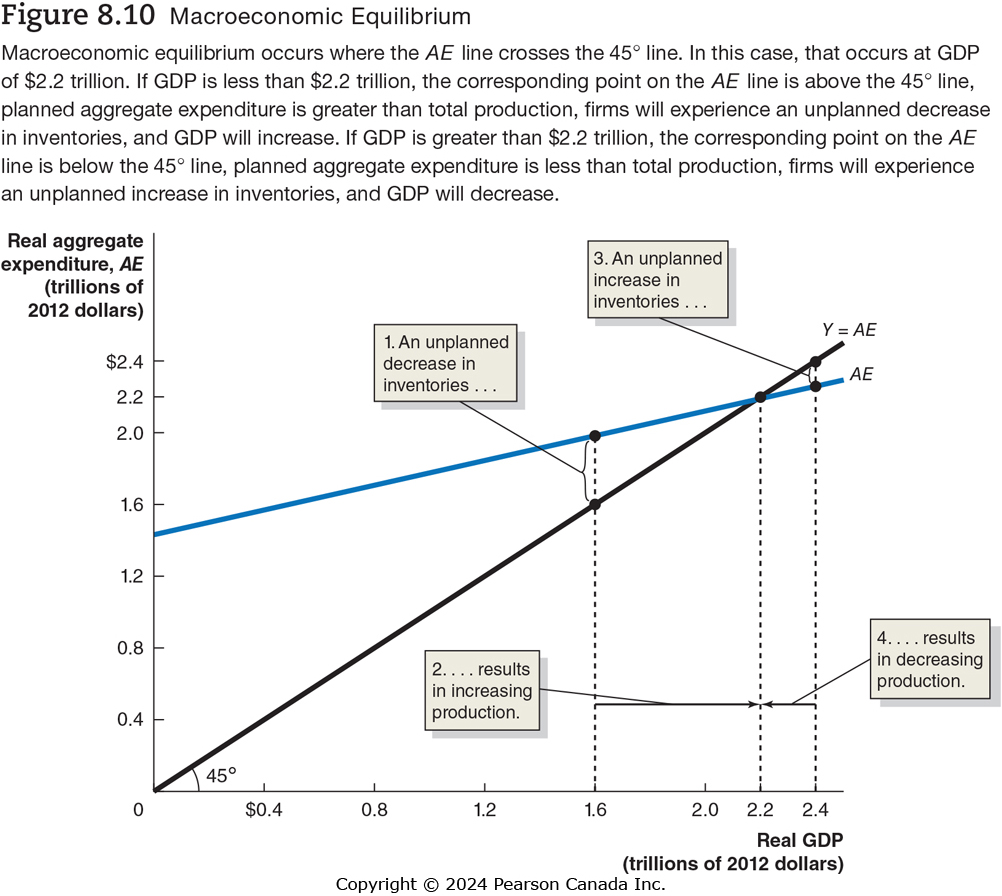
\includegraphics[width=0.6\linewidth]{Fig08-010}.
\end{frame}

\begin{frame}{Figure 8.11 -- A Recession in the 45° Diagram }
\centering
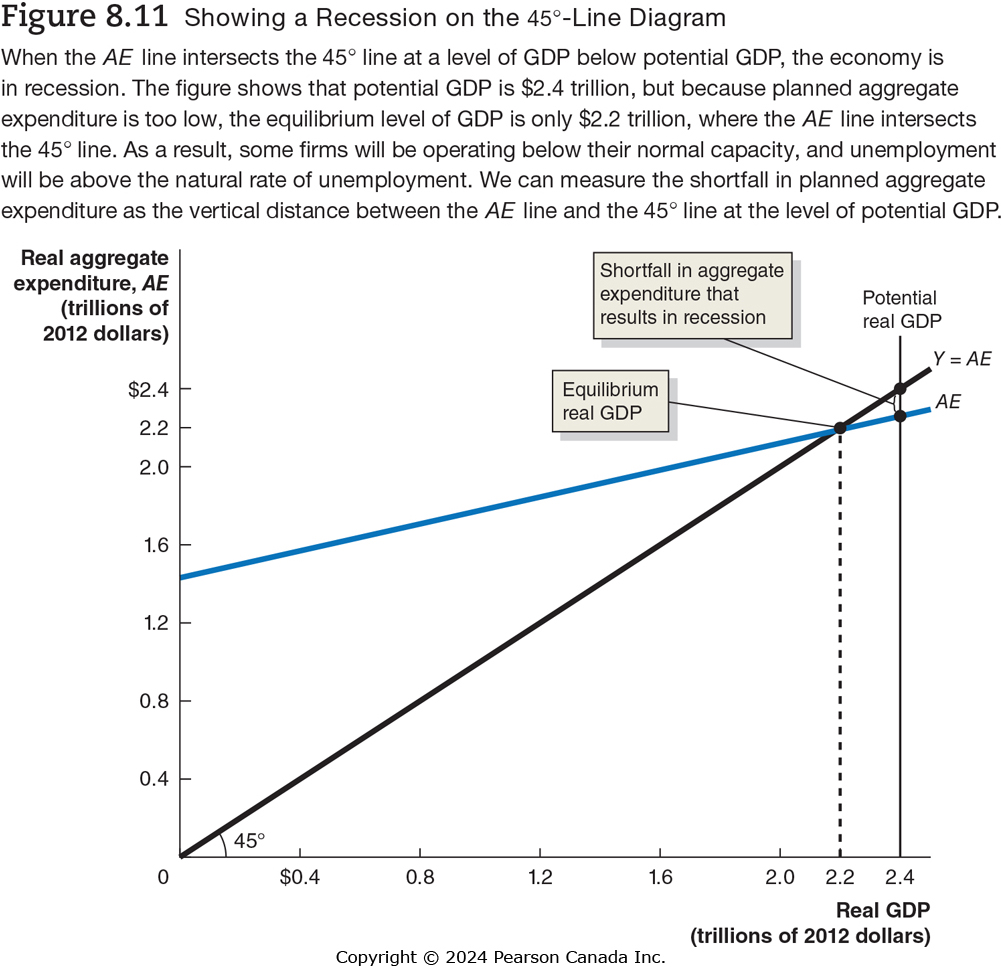
\includegraphics[width=0.6\linewidth]{Fig08-011}.
\end{frame}

\begin{frame}{Inventories and Adjustment}
\transfade
\begin{itemize}[<+->]
  \item Inventories provide the \textbf{signal} that triggers movement toward equilibrium.
  \item If planned AE \(< Y\):
  \begin{itemize}[<+->]
    \item firms accumulate unplanned inventory,
    \item they cut production and employment.
  \end{itemize}
  \item Even when spending returns to normal, firms may first run down the stock of inventories before increasing output.
  \item If planned AE \(> Y\):
  \begin{itemize}[<+->]
    \item inventories are depleted,
    \item firms increase output and hire more workers.
  \end{itemize}
\end{itemize}
\end{frame}

\begin{frame}{Table 8.3 -- Macroeconomic Equilibrium }
\centering
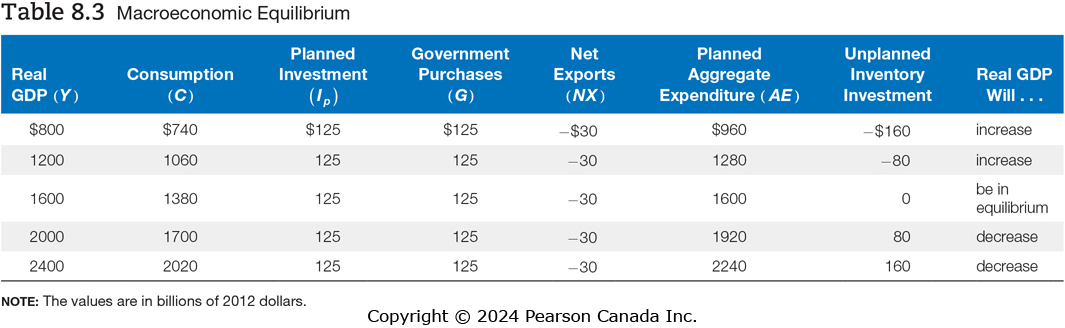
\includegraphics[width=0.94\linewidth]{Tab08-003}.
\end{frame}

% ============================================================
\section{8.4 The Multiplier Effect}
% ============================================================

\begin{frame}{8.4 Learning Objective}
\transfade
\begin{block}{Goal}
Describe the multiplier effect and use the multiplier formula to calculate changes in equilibrium GDP.
\end{block}
\begin{itemize}[<+->]
  \item A small change in \textbf{autonomous expenditure} causes a larger change in equilibrium real GDP.
  \item This amplification is called the \textbf{multiplier effect}.
\end{itemize}
\end{frame}

\begin{frame}{Autonomous vs. Induced Expenditure}
\transfade
\begin{itemize}[<+->]
  \item \textbf{Autonomous expenditure:}
  \begin{itemize}[<+->]
    \item Parts of spending that do not depend on the level of real GDP.
    \item Examples: \(I\), \(G\), \(NX\), and the autonomous part of \(C\).
  \end{itemize}
  \item \textbf{Induced expenditure:}
  \begin{itemize}[<+->]
    \item Spending that \emph{does} depend on real GDP.
    \item For us, this is the part of consumption that changes with income.
  \end{itemize}
  \item Because consumption rises with income, an increase in autonomous spending sets off a chain reaction of additional spending.
\end{itemize}
\end{frame}

\begin{frame}{Figure 8.12 -- The Multiplier Effect }
\centering
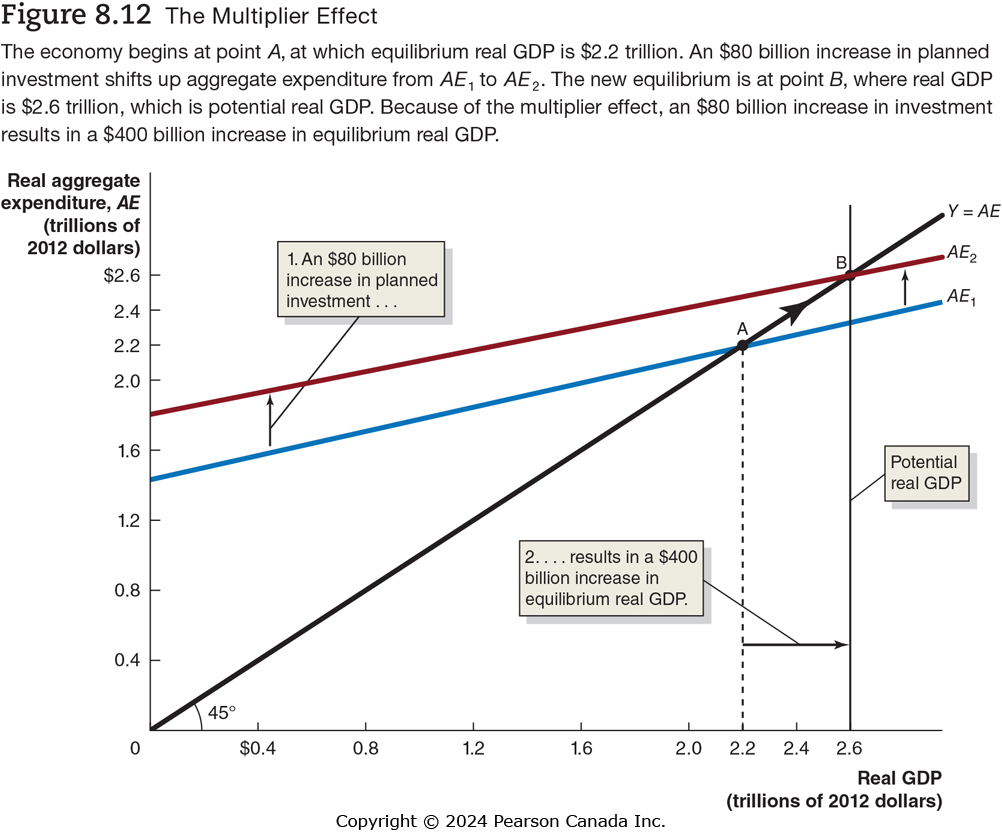
\includegraphics[width=0.6\linewidth]{Fig08-012}.
\end{frame}

\begin{frame}{Table 8.4 -- The Multiplier in Action }
\centering
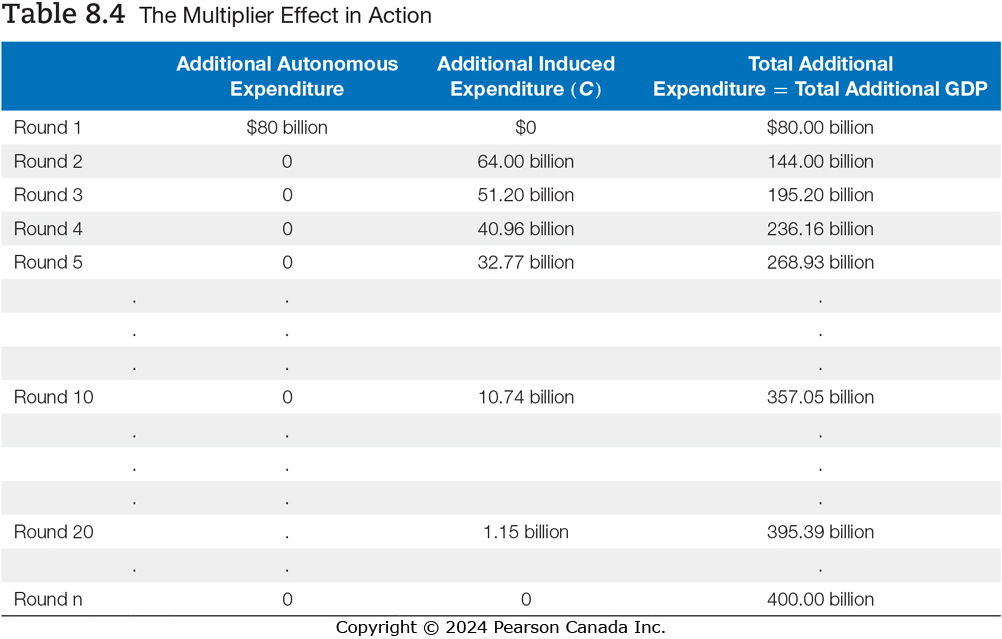
\includegraphics[width=0.68\linewidth]{Tab08-004}.
\end{frame}

\begin{frame}{Eventual Effect of the Multiplier}
\transfade
\begin{itemize}[<+->]
  \item Suppose an initial \$80 billion increase in planned investment.
  \item First round:
  \begin{itemize}[<+->]
    \item AE rises by \$80 billion, so firms increase production by \$80 billion.
  \end{itemize}
  \item Second round:
  \begin{itemize}[<+->]
    \item Income is now higher by \$80 billion.
    \item Households consume \(\text{MPC} \times 80\) billion more.
  \end{itemize}
  \item Third round:
  \begin{itemize}[<+->]
    \item The extra consumption becomes income again, leading to further consumption, and so on.
  \end{itemize}
  \item Eventually, equilibrium GDP rises by \textbf{more} than \$80 billion.
\end{itemize}
\end{frame}

\begin{frame}{Multiplier and MPC: Geometric Series}
\transfade
\begin{itemize}[<+->]
  \item Total change in equilibrium GDP:
  \[
    \Delta Y = \Delta A
      + (\text{MPC}) \Delta A
      + (\text{MPC})^2 \Delta A
      + (\text{MPC})^3 \Delta A
      + \cdots
  \]
  \item Factor out \(\Delta A\):
  \[
    \Delta Y = \Delta A \left[ 1 + \text{MPC}
      + (\text{MPC})^2 + \cdots \right].
  \]
  \item The term in brackets is an infinite geometric series:
  \[
    1 + \text{MPC} + (\text{MPC})^2 + \cdots
    = \frac{1}{1 - \text{MPC}}
    \quad \text{(since } 0 < \text{MPC} < 1\text{)}.
  \]
\end{itemize}
\end{frame}

\begin{frame}{Formula for the Multiplier}
\transfade
\begin{itemize}[<+->]
  \item Therefore:
  \[
    \Delta Y = \frac{1}{1 - \text{MPC}} \times \Delta A.
  \]
  \item The \textbf{multiplier} is:
  \[
    \text{Multiplier} = \frac{1}{1 - \text{MPC}}.
  \]
  \item Example:
  \begin{itemize}[<+->]
    \item If \(\text{MPC} = 0.8\),
    \item multiplier \(= \frac{1}{1 - 0.8} = 5\).
    \item An \$80 billion increase in investment raises equilibrium GDP by:
    \[
      \Delta Y = 5 \times 80 = 400 \text{ billion}.
    \]
  \end{itemize}
\end{itemize}
\end{frame}

\begin{frame}{Summarizing the Multiplier Effect}
\transfade
\begin{itemize}[<+->]
  \item The multiplier works in both directions:
  \begin{itemize}[<+->]
    \item Increases in autonomous expenditure raise GDP by a multiple of the initial change.
    \item Decreases in autonomous expenditure lower GDP by a multiple of the initial change.
  \end{itemize}
  \item The larger the \textbf{MPC}, the larger the multiplier.
  \item Our simple model:
  \begin{itemize}[<+->]
    \item ignores some leakages (e.g., imports, taxes, interest-rate and price changes),
    \item so real-world multipliers are usually smaller than this simple formula suggests.
  \end{itemize}
\end{itemize}
\end{frame}

\begin{frame}{The Paradox of Thrift}
\transfade
\begin{itemize}[<+->]
  \item Long run:
  \begin{itemize}[<+->]
    \item Higher saving can finance more investment and foster growth.
  \end{itemize}
  \item Short run (in the AE model):
  \begin{itemize}[<+->]
    \item If households decide to save more (and consume less),
    \item consumption falls, AE falls,
    \item equilibrium GDP falls, possibly causing a recession.
  \end{itemize}
  \item This tension is known as the \textbf{paradox of thrift}:
  \begin{itemize}[<+->]
    \item What is prudent for individuals can be harmful for the economy in the short run.
  \end{itemize}
  \item In practice, changes in saving also affect interest rates and investment, so the size of this effect is an empirical question.
\end{itemize}
\end{frame}

% ============================================================
\section{8.5 The Aggregate Demand Curve}
% ============================================================

\begin{frame}{8.5 Learning Objective}
\transfade
\begin{block}{Goal}
Understand the relationship between the aggregate demand curve and aggregate expenditure.
\end{block}
\begin{itemize}[<+->]
  \item So far we treated the price level as constant.
  \item Now we ask: what happens to AE when the \textbf{price level changes}?
\end{itemize}
\end{frame}

\begin{frame}{Price Level and Aggregate Expenditure}
\transfade
\begin{itemize}[<+->]
  \item A higher overall price level:
  \begin{itemize}[<+->]
    \item reduces the real value of household wealth,
    \item makes domestic goods more expensive relative to foreign goods,
    \item tends to raise interest rates when the money supply is fixed.
  \end{itemize}
  \item These channels reduce:
  \begin{itemize}[<+->]
    \item consumption,
    \item investment,
    \item and net exports.
  \end{itemize}
  \item Therefore, a higher price level \(\Rightarrow\) lower aggregate expenditure.
  \item A lower price level has the opposite effects.
\end{itemize}
\end{frame}

\begin{frame}{How the Price Level Affects AE}
\transfade
\begin{itemize}[<+->]
  \item \textbf{Wealth effect (on consumption):}
  \begin{itemize}[<+->]
    \item Higher price level reduces real wealth, decreasing consumption.
  \end{itemize}
  \item \textbf{International trade effect (on net exports):}
  \begin{itemize}[<+->]
    \item If domestic prices rise faster than foreign prices, exports fall and imports rise, reducing net exports.
  \end{itemize}
  \item \textbf{Interest rate effect (on investment):}
  \begin{itemize}[<+->]
    \item Higher price level increases money demand.
    \item With a fixed money supply, interest rates rise, reducing investment.
  \end{itemize}
\end{itemize}
\end{frame}

\begin{frame}{Figure 8.13 -- Price Level Changes and Real GDP }
\centering
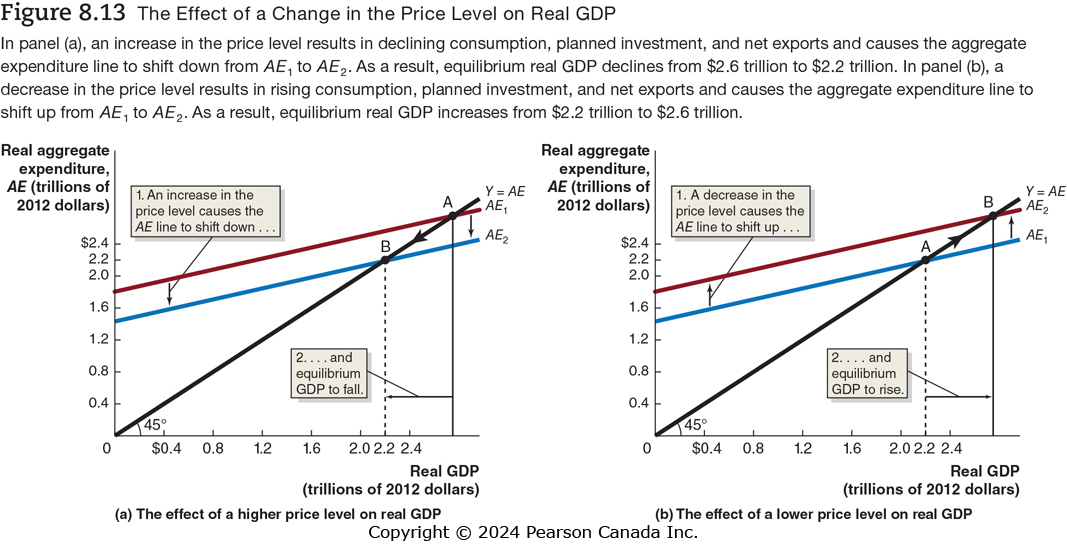
\includegraphics[width=0.97\linewidth]{Fig08-013}.
\end{frame}

\begin{frame}{From AE to the Aggregate Demand Curve}
\transfade
\begin{itemize}[<+->]
  \item For each possible price level, we can:
  \begin{itemize}[<+->]
    \item draw an AE line,
    \item find the corresponding equilibrium real GDP.
  \end{itemize}
  \item Plotting the resulting pairs (price level, equilibrium GDP) gives the:
  \begin{itemize}[<+->]
    \item \textbf{aggregate demand (AD) curve}.
  \end{itemize}
  \item \textbf{Aggregate demand curve:}
  \begin{itemize}[<+->]
    \item relationship between the price level and the quantity of real GDP demanded,
    \item holding constant other factors that affect AE.
  \end{itemize}
\end{itemize}
\end{frame}

\begin{frame}{Figure 8.14 -- The Aggregate Demand Curve }
\centering
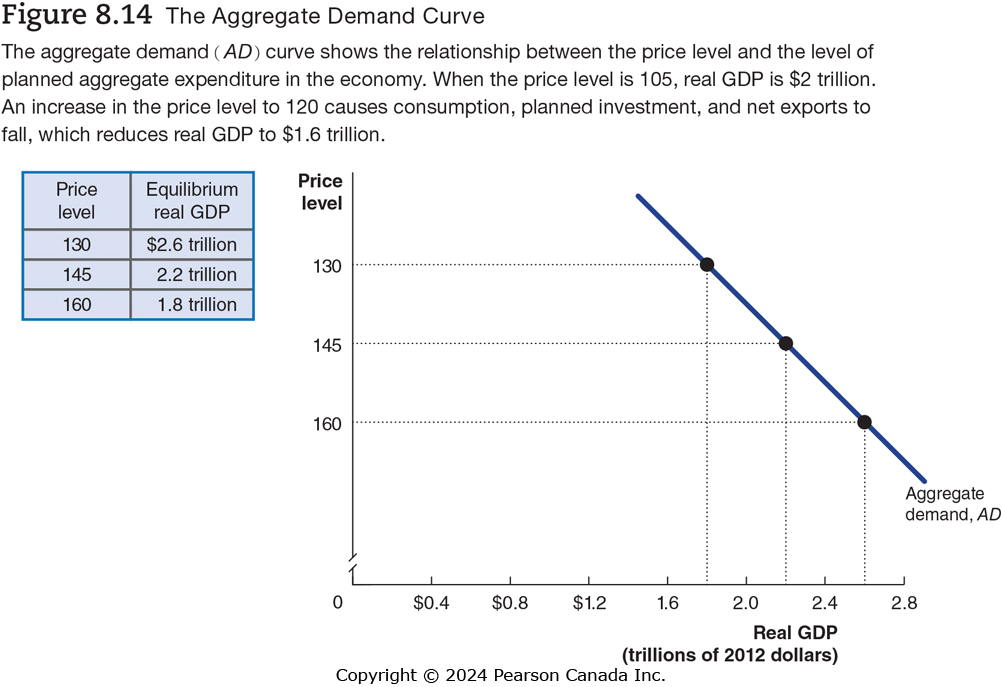
\includegraphics[width=0.9\linewidth]{Fig08-014}.
\end{frame}

\begin{frame}{Common Misconceptions}
\transfade
\begin{itemize}[<+->]
  \item In the 45°-line diagram:
  \begin{itemize}[<+->]
    \item \textbf{Real GDP (Y)} and \textbf{aggregate expenditure (AE)} are conceptually different.
    \item They are equal only at macroeconomic equilibrium.
  \end{itemize}
  \item \textbf{Consumption} is only one component of AE:
  \begin{itemize}[<+->]
    \item AE includes \(C + I + G + NX\).
  \end{itemize}
  \item The aggregate demand curve:
  \begin{itemize}[<+->]
    \item shows the effect of the price level on equilibrium GDP,
    \item not just on consumption.
  \end{itemize}
\end{itemize}
\end{frame}

% ============================================================
\section*{Appendix: Algebra of Macroeconomic Equilibrium}
% ============================================================

\begin{frame}{Appendix: Learning Objective}
\transfade
\begin{block}{Goal}
Apply the algebra of macroeconomic equilibrium to obtain numerical results.
\end{block}
\begin{itemize}[<+->]
  \item Graphs show the \textbf{direction} of change.
  \item Algebraic models allow us to compute \textbf{numerical} changes.
\end{itemize}
\end{frame}

\begin{frame}{Aggregate Expenditure Equations: Example}
\transfade
\begin{itemize}[<+->]
  \item A simple numerical AE model might look like:
  \begin{align*}
    C &= \overline{C} + \text{MPC}\,Y,\\
    I &= \overline{I},\\
    G &= \overline{G},\\
    NX &= \overline{NX},\\
    Y &= C + I + G + NX.
  \end{align*}
  \item The bars indicate \textbf{autonomous} values (do not change with income).
  \item \(\text{MPC}\) is the marginal propensity to consume from national income.
\end{itemize}
\end{frame}

\begin{frame}{Solving the Model: Example}
\transfade
\begin{itemize}[<+->]
  \item Suppose:
  \begin{align*}
    C &= 100 + 0.8Y,\\
    I &= 125,\\
    G &= 125,\\
    NX &= -30.
  \end{align*}
  \item Then the equilibrium condition:
  \[
    Y = C + I + G + NX
  \]
  becomes:
  \[
    Y = 100 + 0.8Y + 125 + 125 - 30.
  \]
  \item Rearranging:
  \[
    Y - 0.8Y = 100 + 125 + 125 - 30
    \quad \Rightarrow \quad
    0.2Y = 320.
  \]
  \item So:
  \[
    Y = \frac{320}{0.2} = 1600.
  \]
\end{itemize}
\end{frame}

\begin{frame}{General Form and Interpretation}
\transfade
\begin{itemize}[<+->]
  \item In general we can write:
  \begin{align*}
    C &= \overline{C} + cY,\\
    I &= \overline{I},\quad
    G = \overline{G},\quad
    NX = \overline{NX},\\
    Y &= C + I + G + NX.
  \end{align*}
  \item Substituting:
  \[
    Y = \overline{C} + cY + \overline{I} + \overline{G} + \overline{NX}.
  \]
  \item Rearranging:
  \[
    Y - cY = \overline{C} + \overline{I} + \overline{G} + \overline{NX}
    \quad \Rightarrow \quad
    (1 - c)Y = A,
  \]
  where \(A\) is total autonomous expenditure.
  \item Therefore:
  \[
    Y = \frac{1}{1 - c} \times A
      = \text{Multiplier} \times \text{Autonomous expenditure}.
  \]
\end{itemize}
\end{frame}

% ============================================================
\section*{Chapter Summary}
% ============================================================

\begin{frame}{Summary}
\transfade
\begin{itemize}[<+->]
  \item The \textbf{AE model} explains short-run equilibrium when the price level is fixed.
  \item Equilibrium occurs where:
  \[
    \text{Planned AE} = Y.
  \]
  \item \textbf{Consumption} is driven by disposable income, wealth, expectations, prices, and interest rates.
  \item \textbf{Investment, government purchases, and net exports} are treated as autonomous in the basic model.
  \item The \textbf{multiplier effect} makes equilibrium GDP more sensitive to changes in autonomous expenditure.
  \item Changes in the \textbf{price level} affect AE through wealth, international trade, and interest rate channels, generating a downward-sloping \textbf{aggregate demand curve}.
\end{itemize}
\end{frame}

\begin{frame}
\centering
\Huge \textbf{Thank you!}
\end{frame}

\end{document}
